%% LyX 1.3 created this file.  For more info, see http://www.lyx.org/.
%% Do not edit unless you really know what you are doing.
\documentclass[english, 12pt]{article}
\usepackage{times}
%\usepackage{algorithm2e}
\usepackage{url}
\usepackage{bbm}
\usepackage[T1]{fontenc}
\usepackage[latin1]{inputenc}
\usepackage{geometry}
\geometry{verbose,letterpaper,tmargin=2.5cm,bmargin=2.5cm,lmargin=2.5cm,rmargin=2.5cm}
\usepackage{rotating}
\usepackage{color}
\usepackage{graphicx}
\usepackage{amsmath, amsthm, amssymb}
\usepackage{setspace}
\usepackage{lineno}
\usepackage{hyperref}
\usepackage{bbm}


%\usepackage{xr}
%\externaldocument{SCT-supp}

\linenumbers
\doublespacing
%\usepackage[authoryear]{natbib}
\usepackage{natbib} \bibpunct{(}{)}{;}{author-year}{}{,}

%Pour les rajouts
\usepackage{color}
\definecolor{trustcolor}{rgb}{0,0,1}

\usepackage{dsfont}
\usepackage[warn]{textcomp}
\usepackage{adjustbox}
\usepackage{multirow}
\usepackage{graphicx}
\graphicspath{{../figures/}}
\DeclareMathOperator*{\argmin}{\arg\!\min}

\let\tabbeg\tabular
\let\tabend\endtabular
\renewenvironment{tabular}{\begin{adjustbox}{max width=\textwidth}\tabbeg}{\tabend\end{adjustbox}}

\makeatletter

%%%%%%%%%%%%%%%%%%%%%%%%%%%%%% LyX specific LaTeX commands.
%% Bold symbol macro for standard LaTeX users
%\newcommand{\boldsymbol}[1]{\mbox{\boldmath $#1$}}

%% Because html converters don't know tabularnewline
\providecommand{\tabularnewline}{\\}

\usepackage{babel}
\makeatother


\begin{document}


\title{Making the most out of Clumping and Thresholding}
\author{Florian Priv\'e,$^{\text{1,}*}$ Bjarni J. Vilhj\'almsson,$^{\text{2}}$ Hugues Aschard$^{\text{3}}$ and Michael G.B. Blum$^{\text{1,}*}$}



\date{~ }
\maketitle

\noindent$^{\text{\sf 1}}$Laboratoire TIMC-IMAG, UMR 5525, Univ.\ Grenoble Alpes, CNRS, La Tronche, France, \\
\noindent$^{\text{\sf 2}}$National Center for Register-based Research, Aarhus University, Denmark. \\
\noindent$^{\text{\sf 3}}$Centre de Bioinformatique, Biostatistique et Biologie Int\'egrative (C3BI), Institut Pasteur, Paris, France,

\noindent$^\ast$To whom correspondence should be addressed.\\

\noindent Contacts:
\begin{itemize}
\item \url{florian.prive@univ-grenoble-alpes.fr}
\item \url{bjv@econ.au.dk}
\item \url{hugues.aschard@pasteur.fr}
\item \url{michael.blum@univ-grenoble-alpes.fr}
\end{itemize}

\newpage

\abstract{

}


%%%%%%%%%%%%%%%%%%%%%%%%%%%%%%%%%%%%%%%%%%%%%%%%%%%%%%%%%%%%%%%%%%%%%%%%%%%%%%%%

\newpage

\section{Introduction}

Clumping and Thresholding (C+T, also called P+T) is a simple technique for computing Polygenic Risk Scores (PRS) based on Genome-Wide Assocation Studies (GWAS) summary statistics, and has been used for more than ten years \cite[]{euesden2014prsice,purcell2009common}.
C+T consists in making a simple sum of allele counts (genotypes), weighted by effect sizes from GWAS summary-statistics, after having restricted the variants included in this sum. The first step consists in keeping only one representative variant by region of linkage disequilibrium (LD) by discarding variants that are too correlated with this particular one. The second step removes variants that are not significant enough, based on p-value from the GWAS summary statistics.
The first step is called ``clumping'' and the second step is called ``thresholding''.
When applying C+T, one has to choose at least 3 hyper-parameters: for clumping, the squared correlation threshold $r_{c}^2$ and the window size $w_c$ of clumping [TODO: RENAME]; for thresholding, the p-value threshold $p_T$.
More often than otherwise, C+T users fix default values for clumping ($r_{c}^2$ of 0.1 or 0.2, and $w_c$ of 250kb or 500kb), and test a few values for $p_T$ between $1$ and $10^{-8}$.
[TABLE REFS]
Moreover, one need to use imputed data to get the same variants between the GWAS and the data to compute the PRS on. People usually use a liberal inclusion of SNPs whatever the imputation accuracy of the variants are, maybe thinking that the more variants they allow in the model, the better would be the prediction.
In this paper, we show that all those parameters are really important, and that choosing those hyper-parameters well could substantially increase the predictive power of C+T over using default parameters.
[TODO: ADD STACKING]
To support our point, we use the UK Biobank data and external summary statistics for similuted and real data analyses \cite[]{bycroft2017genome}.

%%%%%%%%%%%%%%%%%%%%%%%%%%%%%%%%%%%%%%%%%%%%%%%%%%%%%%%%%%%%%%%%%%%%%%%%%%%%%%%%

\section{Material and Methods}

\subsection{Simulations}

We use variants from the UK Biobank imputed dataset that have a minor allele frequency larger than 1\% and an imputation INFO score larger than 0.3. There are almost 10M such variants, we randomly choose 1M of them.
We restrict individuals to the ones referred as of White British ancestry by the UK Biobank and exclude all second individuals in each pair reported as related individuals by the UK Biobank \cite[]{bycroft2017genome}.
335,609 individuals remain and we split them in three sets: one for training (e.g.\ choosing the hyper-parameters) and one for testing (evaluating the models) for which we sample 10,000 different individuals in both sets; and one for computing summary statistics (GWAS) with the 315,609 remaining individuals.

For simulating phenotypes and computing summary statistics, we transform the data into hard calls by randomly sampling hard calls according to imputation probabilities.
For the train and test sets, we use data in dosage format.
This enables us to simulate phenotypes using the ``real'' underlying genotypes as hard calls and use the INFO score (imputation accuracies) reported for the UK Biobank data for the imputed data. [END CLEAR ENOUGH??]

We simulate binary phenotypes with a heritability $h^2 = 50\%$ using a Liability Threshold Model (LTM) with a prevalence of 10\% \cite[]{falconer1965inheritance}. We vary the number of causal variants (100, 10K, or 1M) in order to match a range of genetic architectures from low to high polygenicity.
Liability scores are computed from a model with additive effects only: we compute the liability score of the i-th individual as \(y_i = \sum_{j\in S_\text{causal}} w_j \widetilde{G_{i,j}} + \epsilon_i,\) where $S_\text{causal}$ is the set of causal SNPs, $w_j$ are weights generated from a Gaussian distribution $N(0, h^2 / \vert S_\text{causal} \vert)$, $G_{i,j}$ is the allele count of individual $i$ for SNP $j$, $\widetilde{G_{i,j}}$ corresponds to its standardized version (zero mean and unit variance for all SNPs), and $\epsilon$ follows a Gaussian distribution $N(0, 1 - h^2)$.

To compute summary statistics, we use Cochran-Armitage additive test \cite[]{zheng2012analysis}. Given that we have minimal population structure in our data, this test based on contingency tables is much faster than using a logistic regression with 10 principal components as covariates (40 minutes vs 16 hours) while providing similar effect sizes and Z-scores (Figure \ref{fig:GWAS}).

Each simulation is repeated 10 times.

\subsection{Real summary statistics}

We also investigate prediction using real summary statistics from published GWAS, summarized in table \ref{tab:sumstats} \cite[]{buniello2018nhgri}.
[DATA??]

\begin{table}[h]
\caption{\label{tab:sumstats}}
\vspace*{0.5em}
\centering
\begin{tabular}{|l|c|c|c|c|c|}
  \hline
Trait & GWAS size (cases / controls) & Number of SNPs & Citation & Download \\
  \hline
Breast cancer &  &  & \cite{michailidou2017association} & \href{ftp://ftp.ebi.ac.uk/pub/databases/gwas/summary_statistics/MichailidouK_29059683_GCST004988}{link} \\
Prostate cancer & 79,148 / 61,106 &  & \cite{schumacher2018association} & \href{http://practical.icr.ac.uk/blog/?page_id=8164}{link} \\
Coronary artery disease &  &  & \cite{van2018identification} & \href{ftp://ftp.ebi.ac.uk/pub/databases/gwas/summary_statistics/vanderHarstP_29212778_GCST005194}{link} \\
Inflammatory bowel disease \\
Rheumatoid Arthritis \\
Type 2 diabetes  \\
Mean arterial pressure?? \\
Intelligence / EA?? \\
   \hline
\end{tabular}
\end{table}

%%%%%%%%%%%%%%%%%%%%%%%%%%%%%%%%%%%%%%%%%%%%%%%%%%%%%%%%%%%%%%%%%%%%%%%%%%%%%%%%

\section{Results}



%%%%%%%%%%%%%%%%%%%%%%%%%%%%%%%%%%%%%%%%%%%%%%%%%%%%%%%%%%%%%%%%%%%%%%%%%%%%%%%%

\section{Discussion}




%%%%%%%%%%%%%%%%%%%%%%%%%%%%%%%%%%%%%%%%%%%%%%%%%%%%%%%%%%%%%%%%%%%%%%%%%%%%%%%%

\section*{Acknowledgements}

Authors acknowledge LabEx PERSYVAL-Lab (ANR-11-LABX-0025-01) and ANR project FROGH (ANR-16-CE12-0033). Authors also acknowledge the Grenoble Alpes Data Institute that is supported by the French National Research Agency under the ``Investissements d'avenir'' program (ANR-15-IDEX-02).
This research has been conducted using the UK Biobank Resource under Application Number 25589.

%%%%%%%%%%%%%%%%%%%%%%%%%%%%%%%%%%%%%%%%%%%%%%%%%%%%%%%%%%%%%%%%%%%%%%%%%%%%%%%%

\newpage

\bibliographystyle{natbib}
\bibliography{refs}


\newpage
\section*{Supplementary Data}

\renewcommand{\thefigure}{S\arabic{figure}}
\setcounter{figure}{0}
\renewcommand{\thetable}{S\arabic{table}}
\setcounter{table}{0}

\begin{figure}[htb]
\centerline{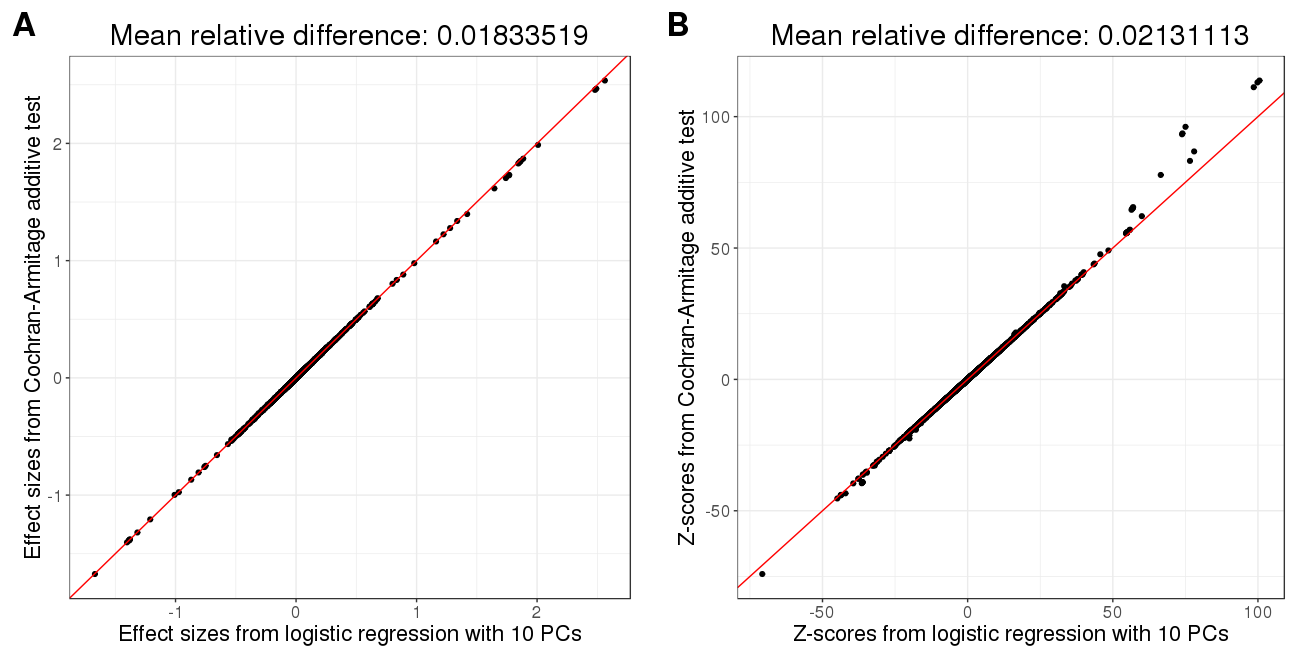
\includegraphics[width=0.95\textwidth]{equivalence.png}}
\caption{Comparison of estimated effect sizes (\textbf{A}) and Z-scores (\textbf{B}) if computed using a logistic regression with 10 principal components as covariates, or with a simple Cochran-Armitage additive test. Phenotypes were simulated using 100 causal SNPs only, allowing for large effects.}
\label{fig:GWAS}
\end{figure}

\end{document}
